\section{共享单车的背景与意义}
\subsection{共享单车的背景}
自2006年出现首家专业租车网站以来,中国在线出行服务行业经历了“线下重资产+线上服务”向“互联网+共享经济/轻资产重服务”的转变,同时也实现了PC端向移动端使用场景的转变;2012年起移动端出行服务模式大量涌现,主流服务包括租车、拼车、代驾、出租车、专车(快车)与分时租赁等,其中,专/快车、共享单车等共享出行服务成为其主流服务\cite{陈正豪2017从三个方面看一看共享单车的行业背景}。可以将在线出行服务发展历程归结为三个转变:
\begin{enumerate}
    \item 运营模式:从“线下重资产+线上服务”转向“互联网+共享经济/轻资产重服务”;
    \item 使用场景:经历了PC端到移动端的转变,这和智能手机的普及和渗透是离不开的;
    \item 量级:2012年起移动端出行服务模式大量涌现。
\end{enumerate}

共享单车的发展离不开公共自行车管理系统的发展,从1965年第一代公共自行车系统在荷兰问世,该系统采用完全免费,不上锁且无人监管,市民可随意取用,但无法解决自行车偷盗损毁问题;在这之后的1995年第二代公共自行车系统又出现了:固定存取地点,投币开锁,但管理难度较大;再到20世纪90年代末第三代基于信息技术与会员制管理,这一模式成为了当前政府的一个主流模式;终于在2010年,美国Social Bicycles创意性地提出了借助手机APP和GPS定位,快速租用归还的无桩模式运营,这便是共享单车的雏形\cite{陈正豪2017从三个方面看一看共享单车的行业背景,刘亚楠2017共享单车发展研究分析}。

作为在线出行行业的主流服务,共享出行包含专车、快车等网约车服务,分时租赁服务,以及2016年火爆市场的共享单车服务;相比网约车的专/快车及顺风车,共享单车解决了用户“最后一公里”的出行问题,节约用户等车的时间成本及服务的费用成本;相比分时租赁,共享单车使用方便,取还车灵活,使用性价比高,目前共享单车用户覆盖率增长迅速,远超分时租赁用户群体\cite{陈正豪2017从三个方面看一看共享单车的行业背景,李琨浩2017基于共享经济视角下城市共享单车发展对策研究}。

采用PEST分析法可知,共享单车的发展环境主要得益于政府、经济、社会和技术四方面\cite{陈正豪2017从三个方面看一看共享单车的行业背景}:
\begin{enumerate}
    \item 政府层面:强调改善出行环境,规范出行规则,鼓励资本合作,推动智能创造;
    \item 经济层面:整体经济呈温和上升趋势,智能手机渗透率增长迅速;
    \item 社会层面:空气污染严重,城市交通拥堵等出行问题亟待解决;
    \item 技术层面:智能手机与4G网络的普及,物联网技术发展,为共享单车的普及搭建了良好的平台。
\end{enumerate}

我们可以对共享单车的用户画像进行分析:
\begin{enumerate}
    \item 性别男性用户偏多,摩拜男性用户更多;
    \item 摩拜和OFO以年轻用户为主,相对来看永安行用户年龄偏大,主要还是以年轻用户为主。
    \item 新兴共享单车以一线城市用户为主,市政单车在二三线渗透更深。
    \item 用户设备以华为、三星等为主,摩拜用户相对高端。
\end{enumerate}

最后我们总结出这样一个用户画像(如图~\ref{F:user-portrait}):共享单车主要用户为中高等收入且追求健康生活方式的中青年男性\cite{陈正豪2017从三个方面看一看共享单车的行业背景},。

\begin{figure}[htbp]
    \centering
    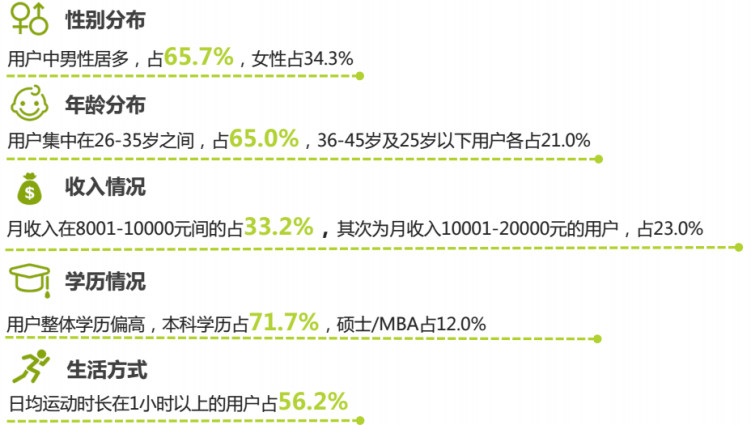
\includegraphics[width=.75\textwidth]{user-portrait}
    \caption{共享单车用户画像}\label{F:user-portrait}
\end{figure}


\subsection{共享单车数据的意义}
除了共享单车系统在现实世界中的有趣应用外,由系统产生的数据也吸引着研究人员从事相关方面的研究。共享单车在使用时间与起止位置上都是精确记录的,在这一点上不像是诸如公共汽车、地铁等的交通,而这一特性使得共享单车系统可以在一定程度上作为虚拟传感器网络,可用于感知城市范围内的转移。因此,可以通过对数据的探索从而预测城市内大多数的重要事件。\cite{范东旭刘威2018沈阳市共享单车大数据分析与发展对策研究,data}
